\newpage
\section{Cấu trúc lớp vỏ electron của nguyên tử}
\begin{mtbh}
	\begin{itemize}
		\item Trình bày và so sánh được mô hình của Rutherford - Bohr với mô hình hiện đại mô tả sự chuyển động của electron trong nguyên tử
		\item Nêu được khái niệm vể orbital nguyên tử (A0), mô tả được hình dạng của AO (s, p), số lượng electron trong $1 \mathrm{~A} 0$.
		\item Trình bày được khái niệm lớp, phân lớp electron và mối quan hệ vể số lượng phân lớp trong một lớp. Liên hệ được vể số lượng A0 trong một phân lớp, trong một lớp.
		\item Viết được cấu hình electron nguyên tử theo lớp, phân lớp electron và theo ô orbital khi biết số hiệu nguyên tử $Z$ của 20 nguyên tố đẩu tiên trong bảng tuẩn hoàn.
		\item Dựa vào đặc điểm cấu hình electron lớp ngoài cùng của nguyên tử dự đoán được tính chất hoá học cơ bản (kim loại hay phi kim) của nguyên tố tương ứng. 
	\end{itemize}
\end{mtbh}

\begin{kd}
	Trong một lớp học để tiện cho việc quản lý và tổ chức học tập, các em học sinh được xếp theo dãy , mỗi dãy gồm nhiều tổ, mỗi tổ gồm nhiều bàn và mỗi bàn gồm 3-4 em học sinh. Vậy thì khi các electron chuyển động xung quanh hạt nhân chứng sắp xếp như thế nào? Để tìm hiểu rõ chúng ta đi vào bài học hôm nay.
\end{kd}
\newpage
\subsection{Sự chuyển động của electron trong nguyên tử}
\subsubsection{Sự chuyển động của electron trong nguyên tử}
\begin{hoivadap}
	Quan sát hình \ref{fig:mhntbo} và \ref{fig:mhnthd} , so sánh điểm giống và khác nhau giữa mô hình Rutherford - Bohr với mô hình hiện đại mô tả sự chuyến động của electron trong nguyên tử.\\
		\begin{center}
		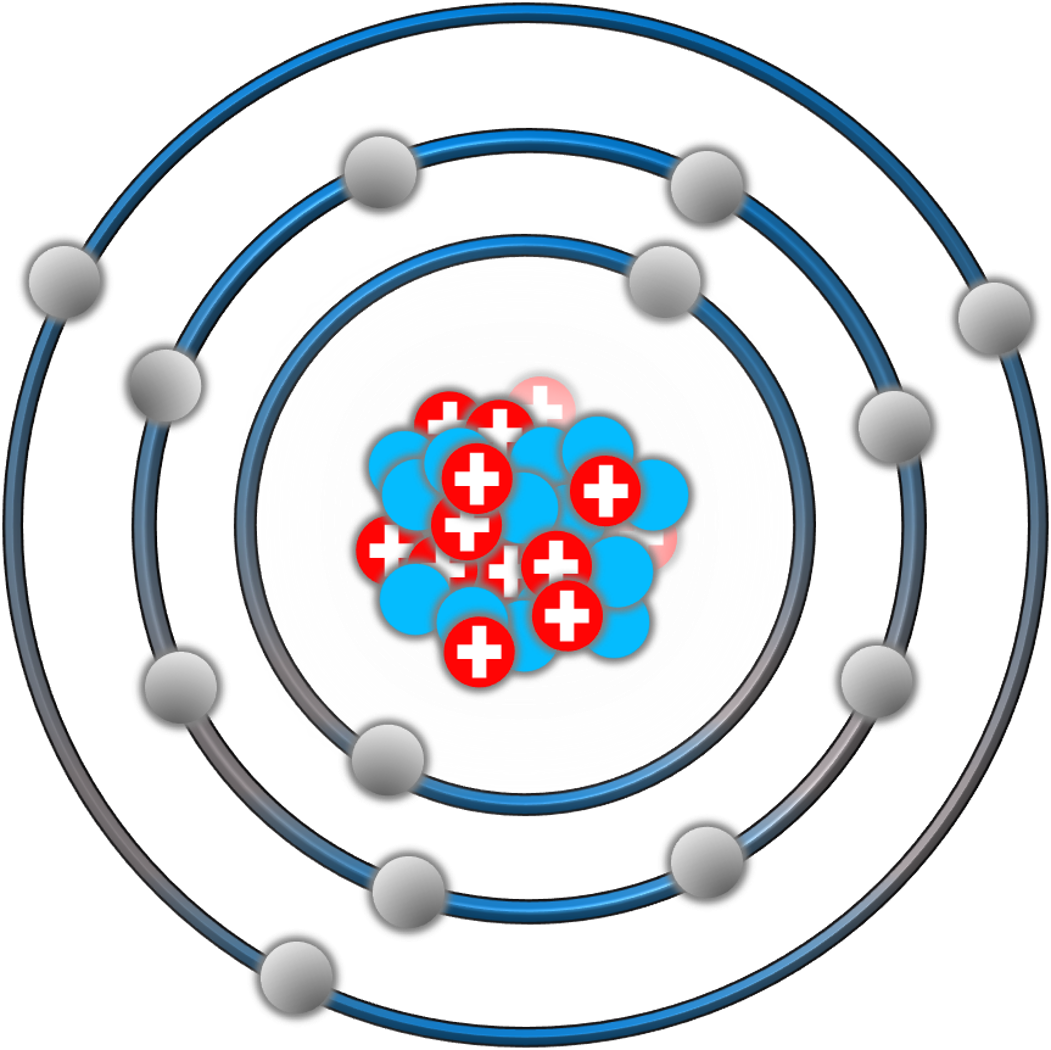
\includegraphics[width=3cm]{Images/anhminhoa/mohinhntbor.png}
		\captionof{figure}{Mô hình nguyên tử Rutherford - Bohr}
		\label{fig:mhntbo}
		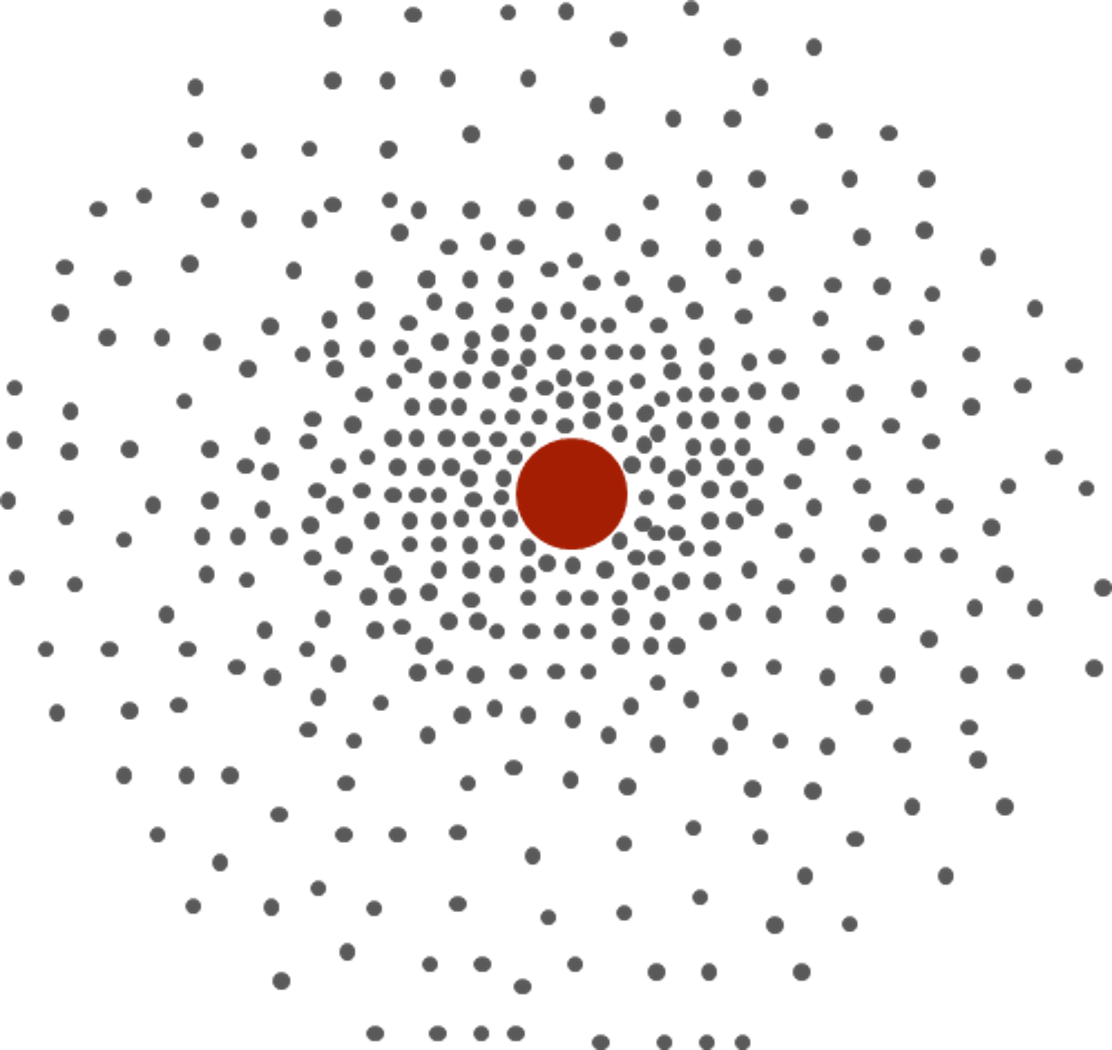
\includegraphics[width=3cm]{Images/anhminhoa/Mohinhnguyentuhiendai.png}
		\captionof{figure}{Mô hình nguyên tử hiện đại}
		\label{fig:mhnthd}
		\end{center}
\huongdan{
\begin{tabular}{|C{.25\textwidth}|L{0.65\textwidth}|}
\hline
\rowcolor{\mycolor!50!white} \multicolumn{1}{|c|}{ \sffamily\textbf{Mô hình} } & \multicolumn{1}{c|}{ \sffamily\textbf{Nội dung} } \\
\hline 
	Rutherford-Bohr &\makecell[l]{- Chưa có hạt neutron \\- Các electron quay xung quanh hạt nhân theo từng quỹ đạo\\ tròn ổn định, trong đó mỗi quỹ đạo có một mức năng lượng\\ xác định.}\\
\hline	
\makecell[c]{Hiện đại\\(Đám mây electron)} & \makecell[l]{- Đã tìm ra hạt neutron \\- Các electron chuyển độngh rất nhanh xung quanh hạt nhân\\ không theo một quỹ đạo xác định và tạo thành một đám mây\\ mang điện tích âm.}\\
\hline
\end{tabular}
}
\end{hoivadap}

\begin{emcobiet}
	Mô hình của Rutherford được gọi là mô hình mẫu hành tinh nguyên tử.
\end{emcobiet}
\subsubsection{Tìm hiểu về orbital nguyên tử}

\begin{dngsnd}
	\begin{itemize}
		\item \indam{Orbital nguyên tử} (Atomic Orbital, viết tắt $\mathrm{AO}$ ) là khu vực không gian xung quanh hạt nhân nguyên tử mà tại đó xác suất tìm thấy electron là lớn nhất (khoảng $90 \%$ ).
		\item Dựa trên sự khác nhau  về hình dạng và sự định hướng trong không gian của các orbital, người ta phân thành orbital s, orbital p, orbital d,orbital f
	\end{itemize}
\end{dngsnd}
Dưới đây là hình ảnh một số AO-s và AO-d (xem hình \ref{fig:hinhdangAO})\\
\begin{tikzpicture}
	% Định dạng cho cột của bảng
	\tikzset{%
		mynode/.style={%
		    ultra thick,
			minimum height=0.65cm,
			align=center,
			font=\sffamily
		},
		mymatrix/.style={%
			matrix of nodes,
			nodes={mynode},
			row 1/.style={%
				nodes={%
					fill=\mycolor!40!white,
					text centered,
					font=\bfseries\sffamily
				}
			},
			column 1/.style={%
				nodes={minimum width=0.25\textwidth}
			},
			column 2/.style={%
				nodes={minimum width=0.25\textwidth}
			},
			column 3/.style={%
				nodes={minimum width=0.25\textwidth}
			},
			column 4/.style={%
				nodes={minimum width=0.25\textwidth}
			}
		}
	}
	\matrix(Bang)[mymatrix]{%
	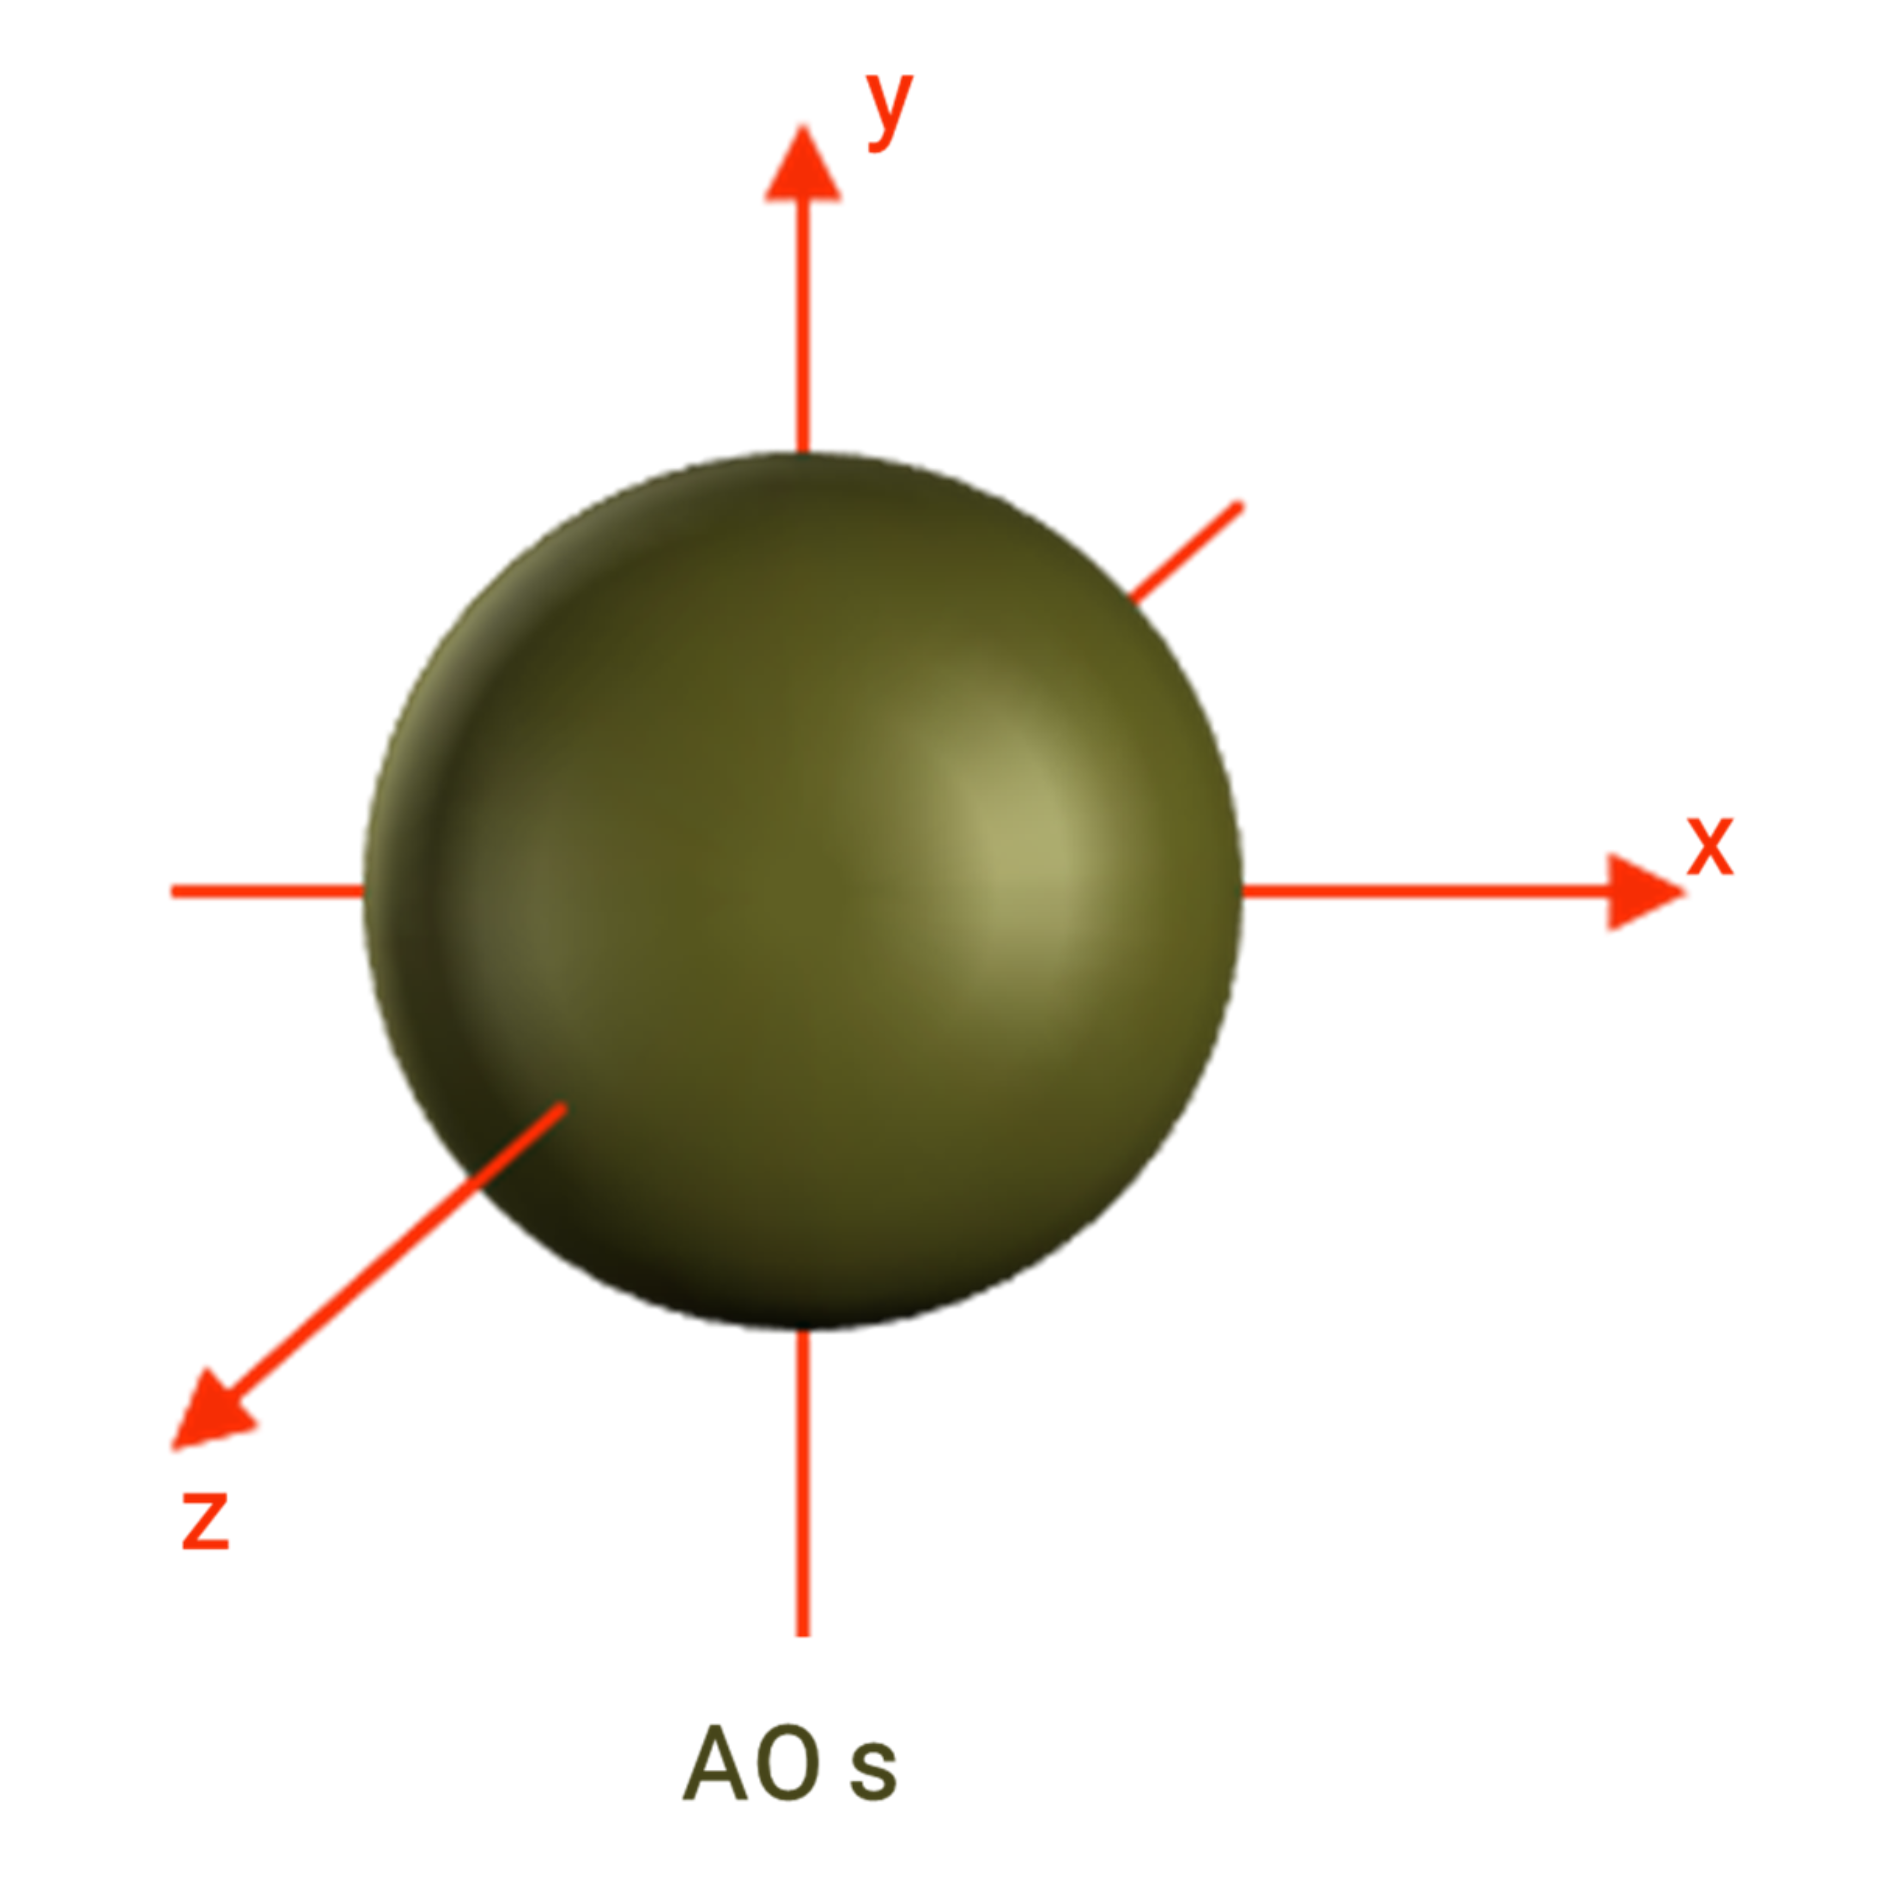
\includegraphics[width=3cm]{Images/anhminhoa/S.png}  & 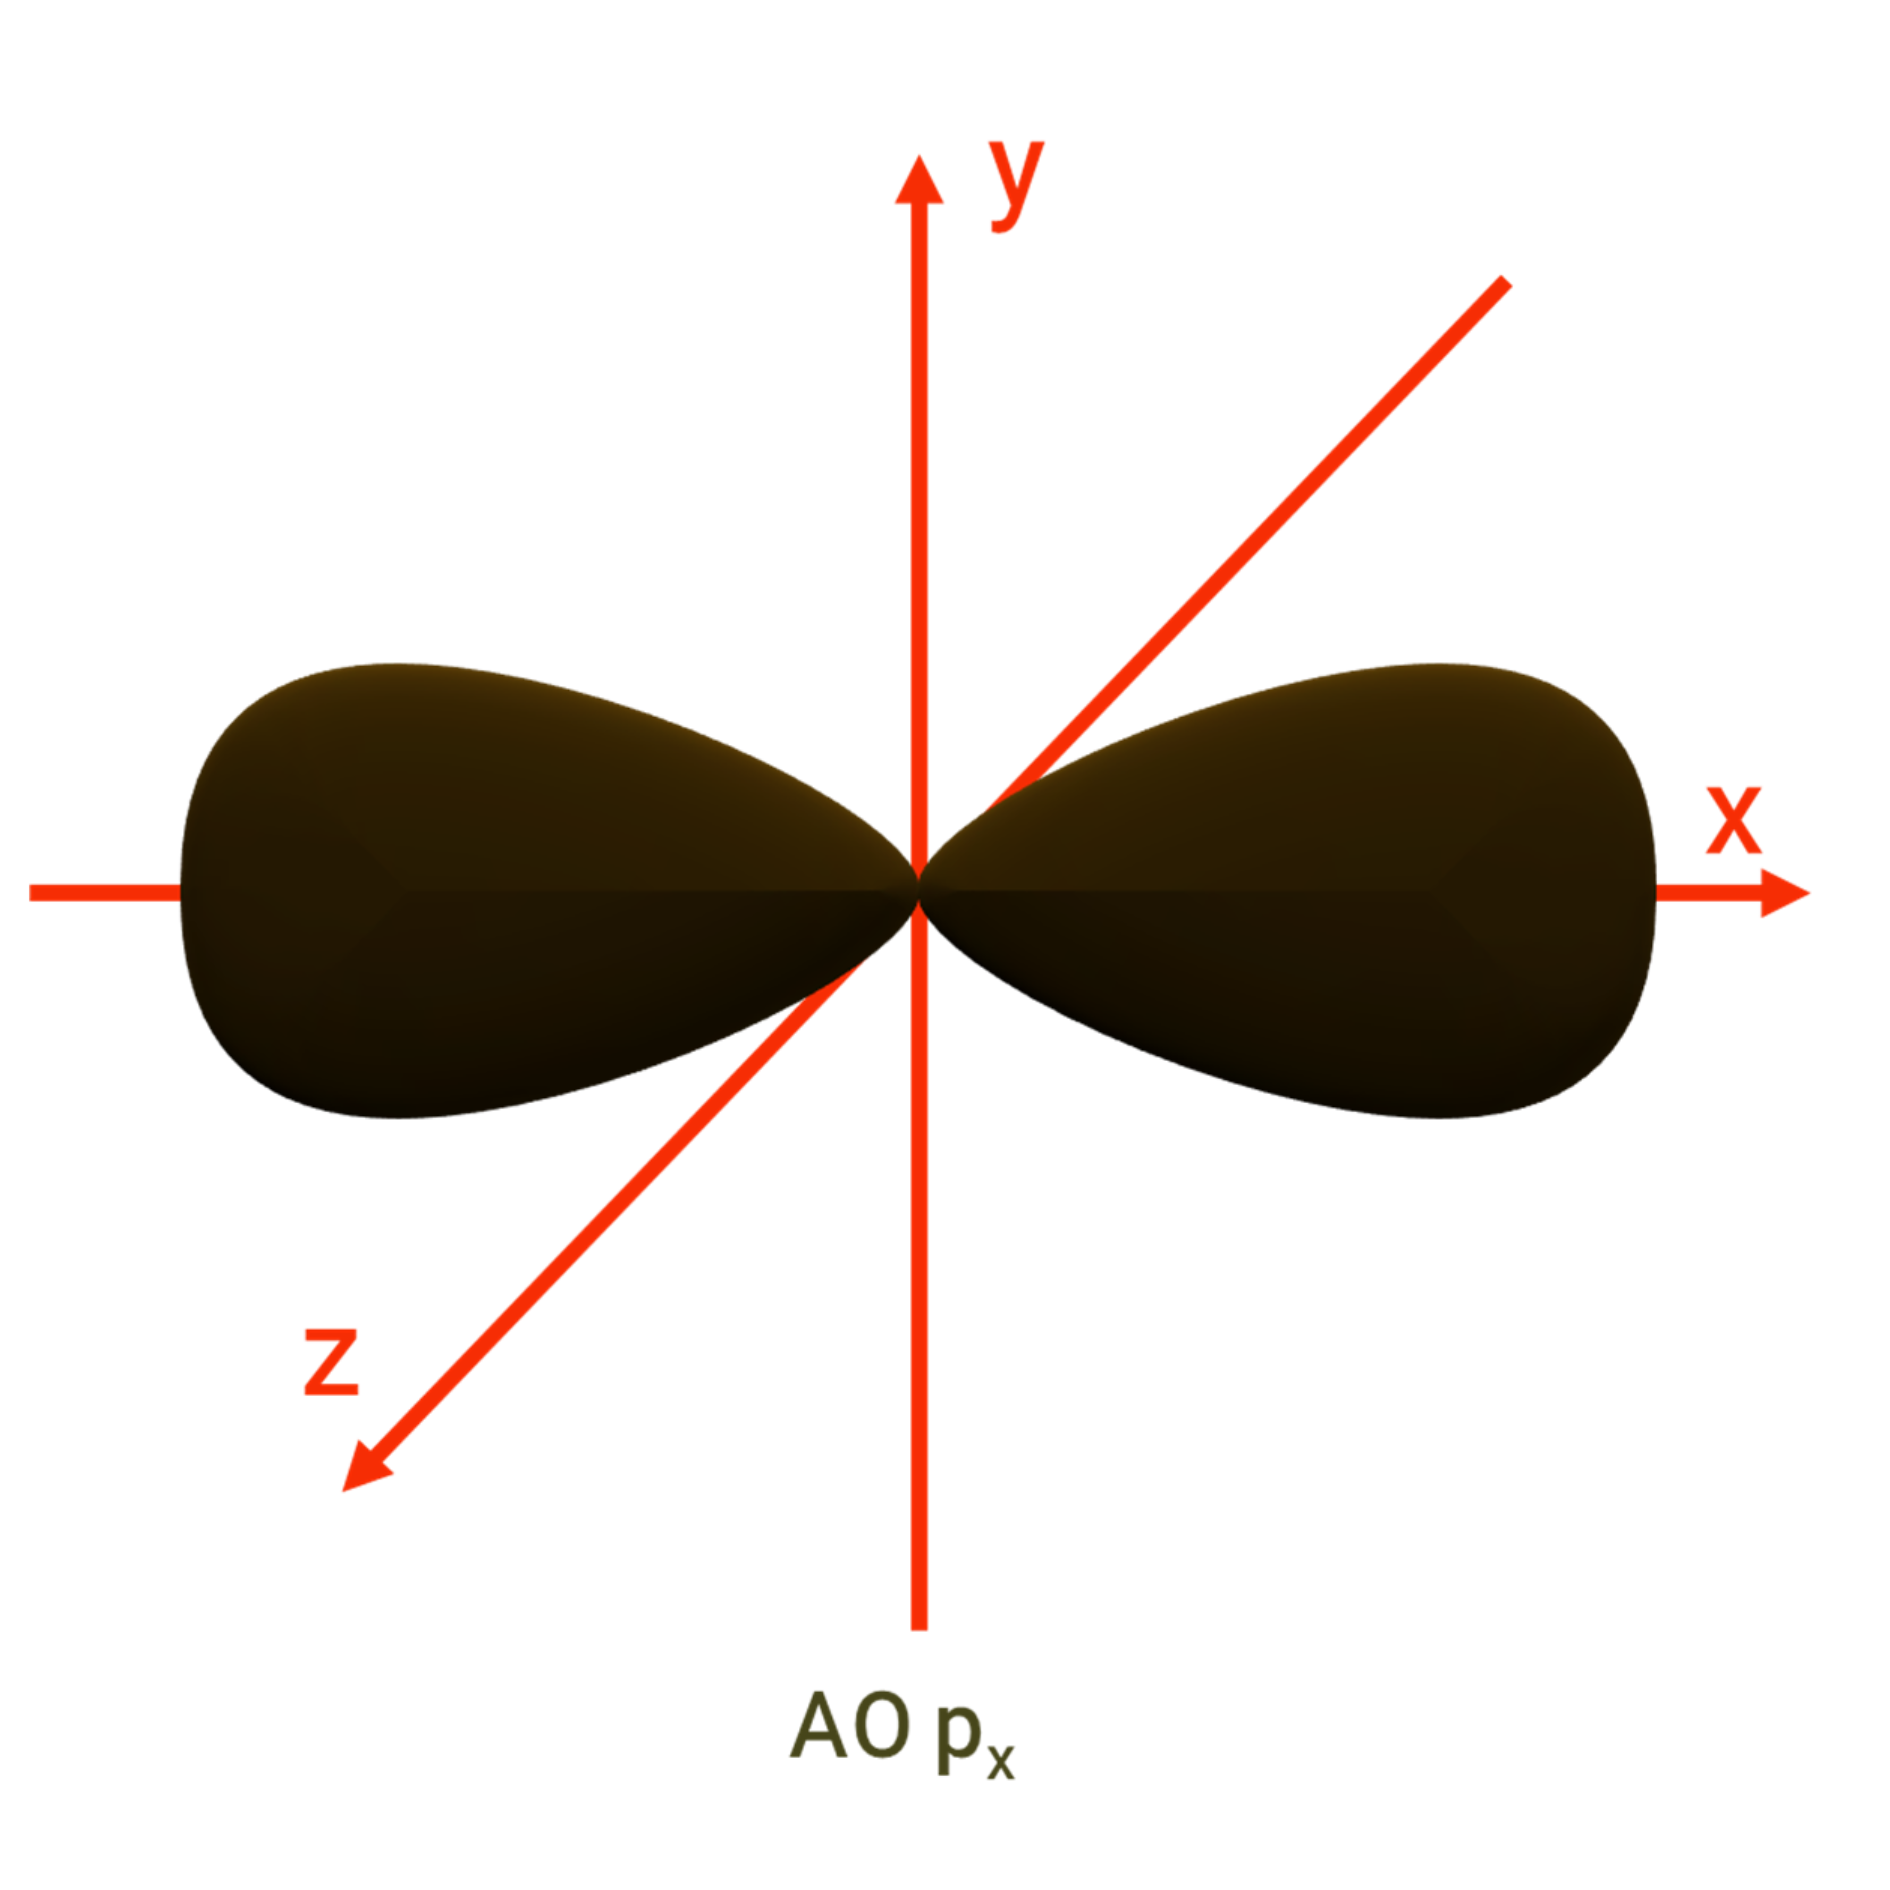
\includegraphics[width=3cm]{Images/anhminhoa/Px.png} & 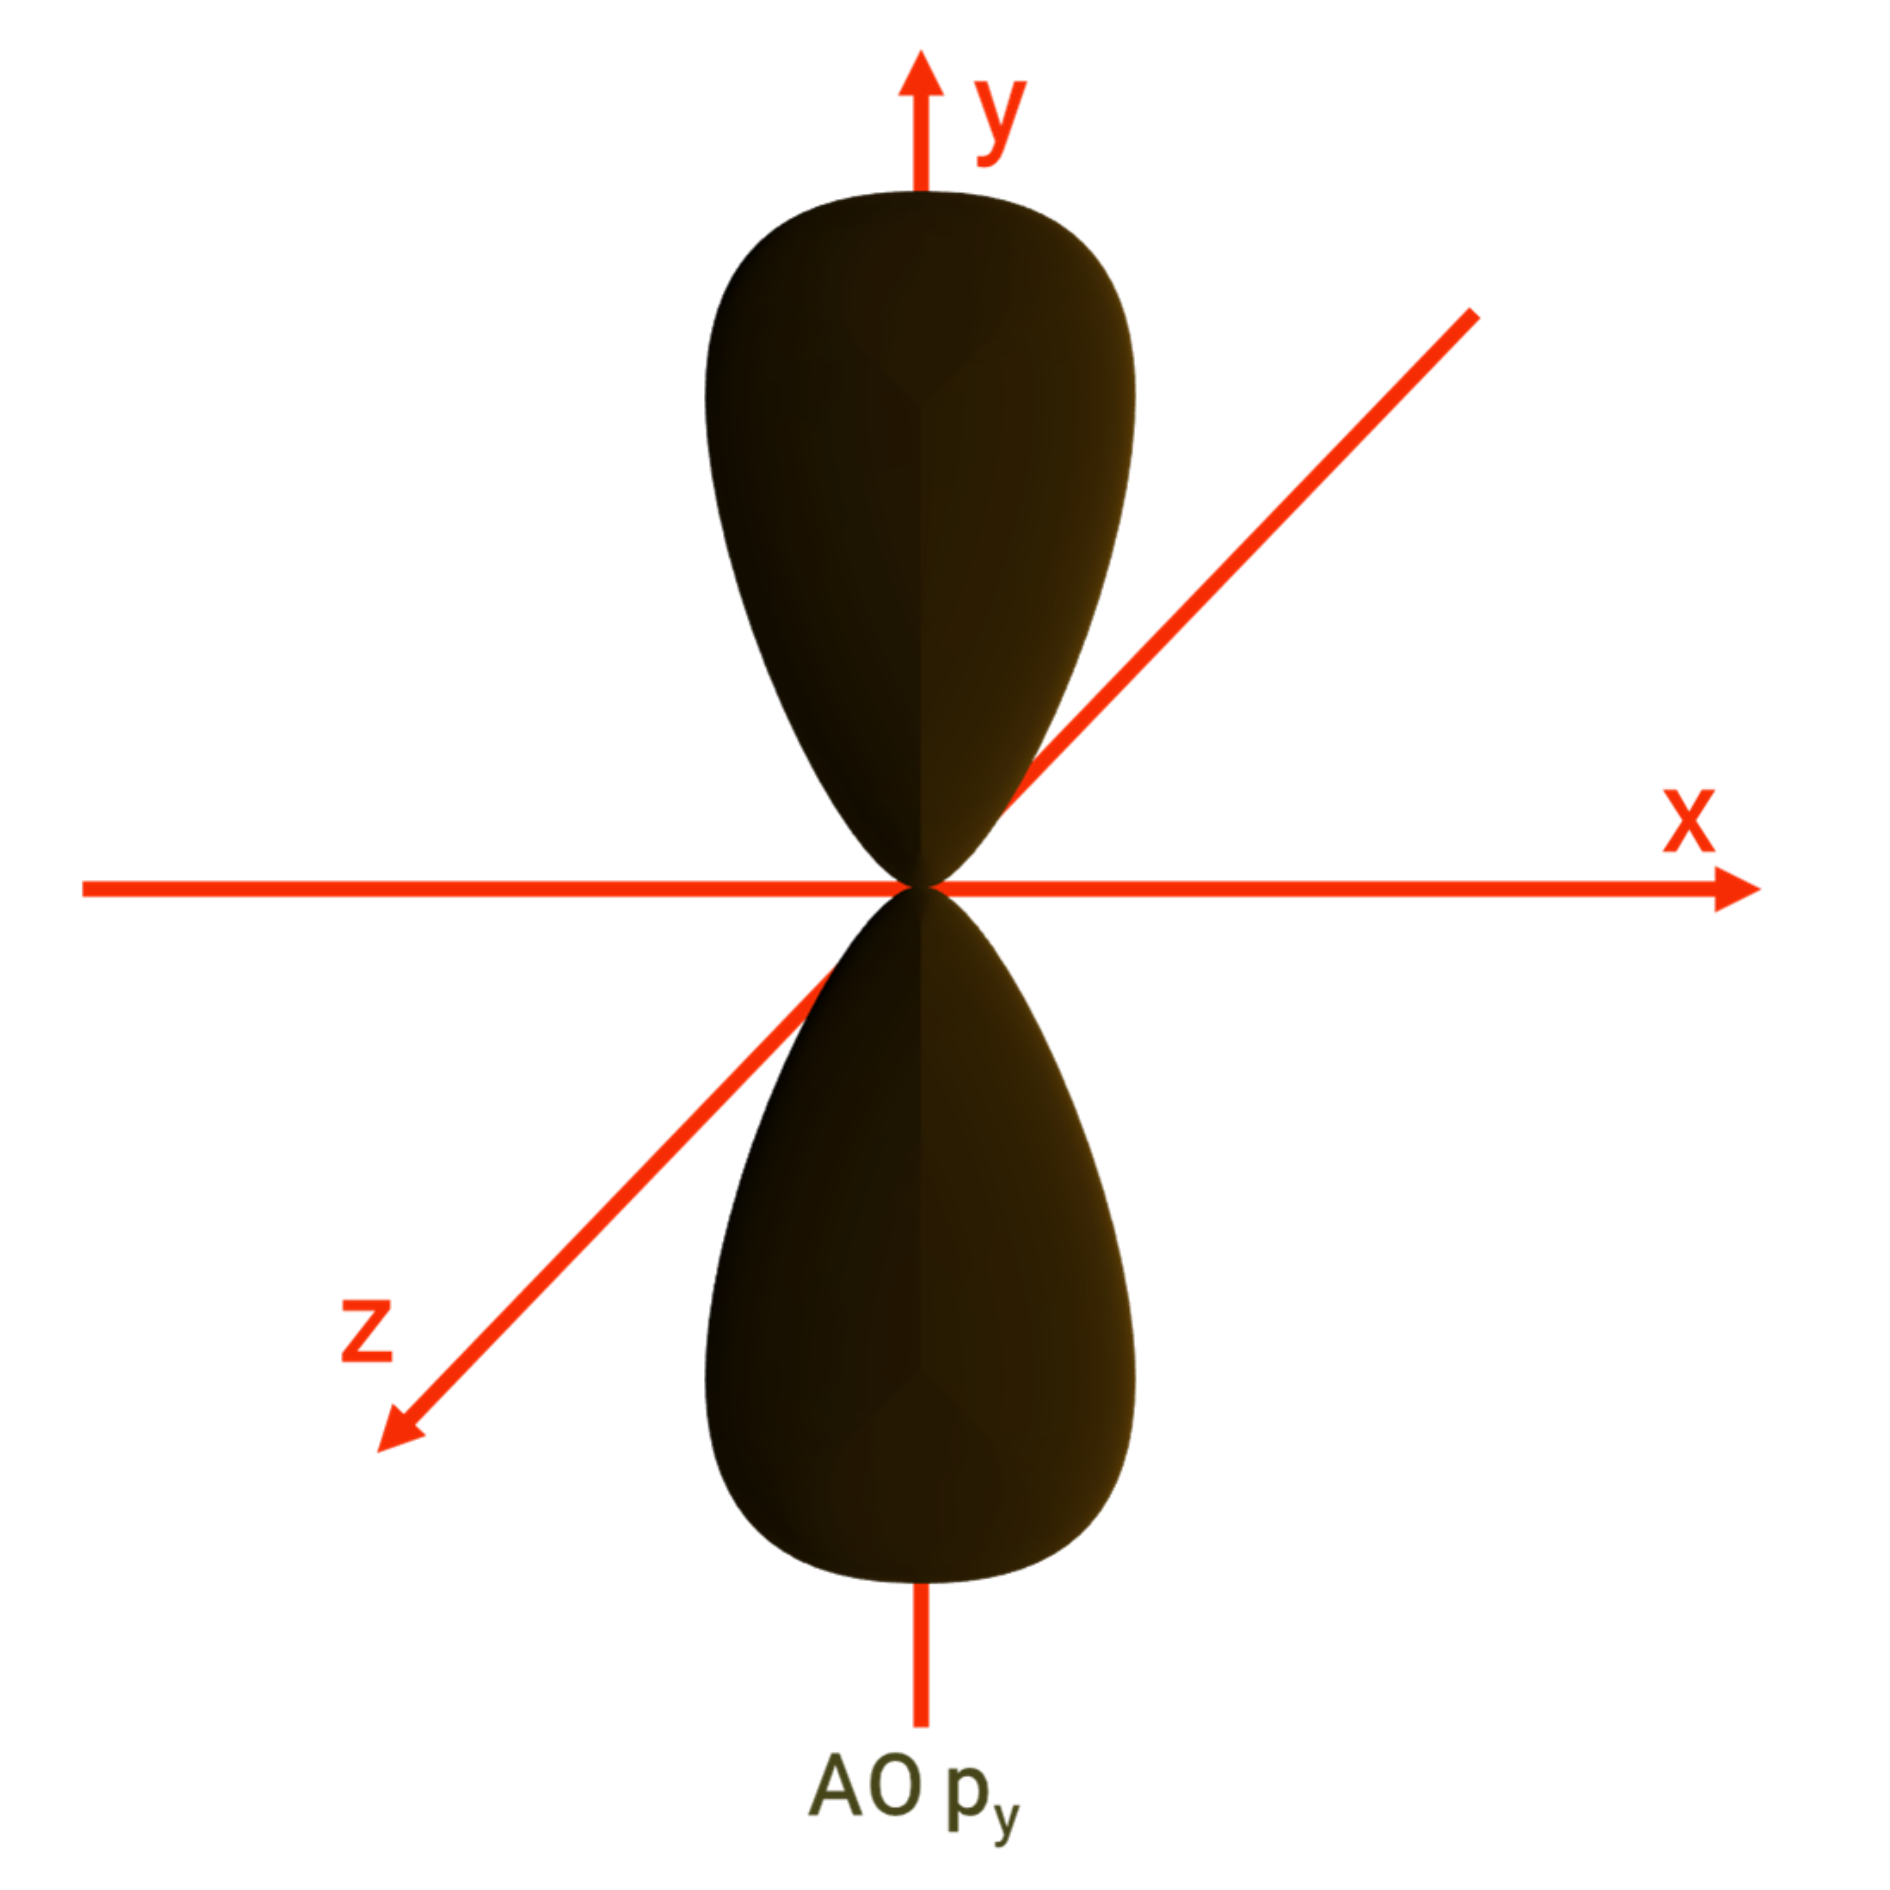
\includegraphics[width=3cm]{Images/anhminhoa/Py.png} &
	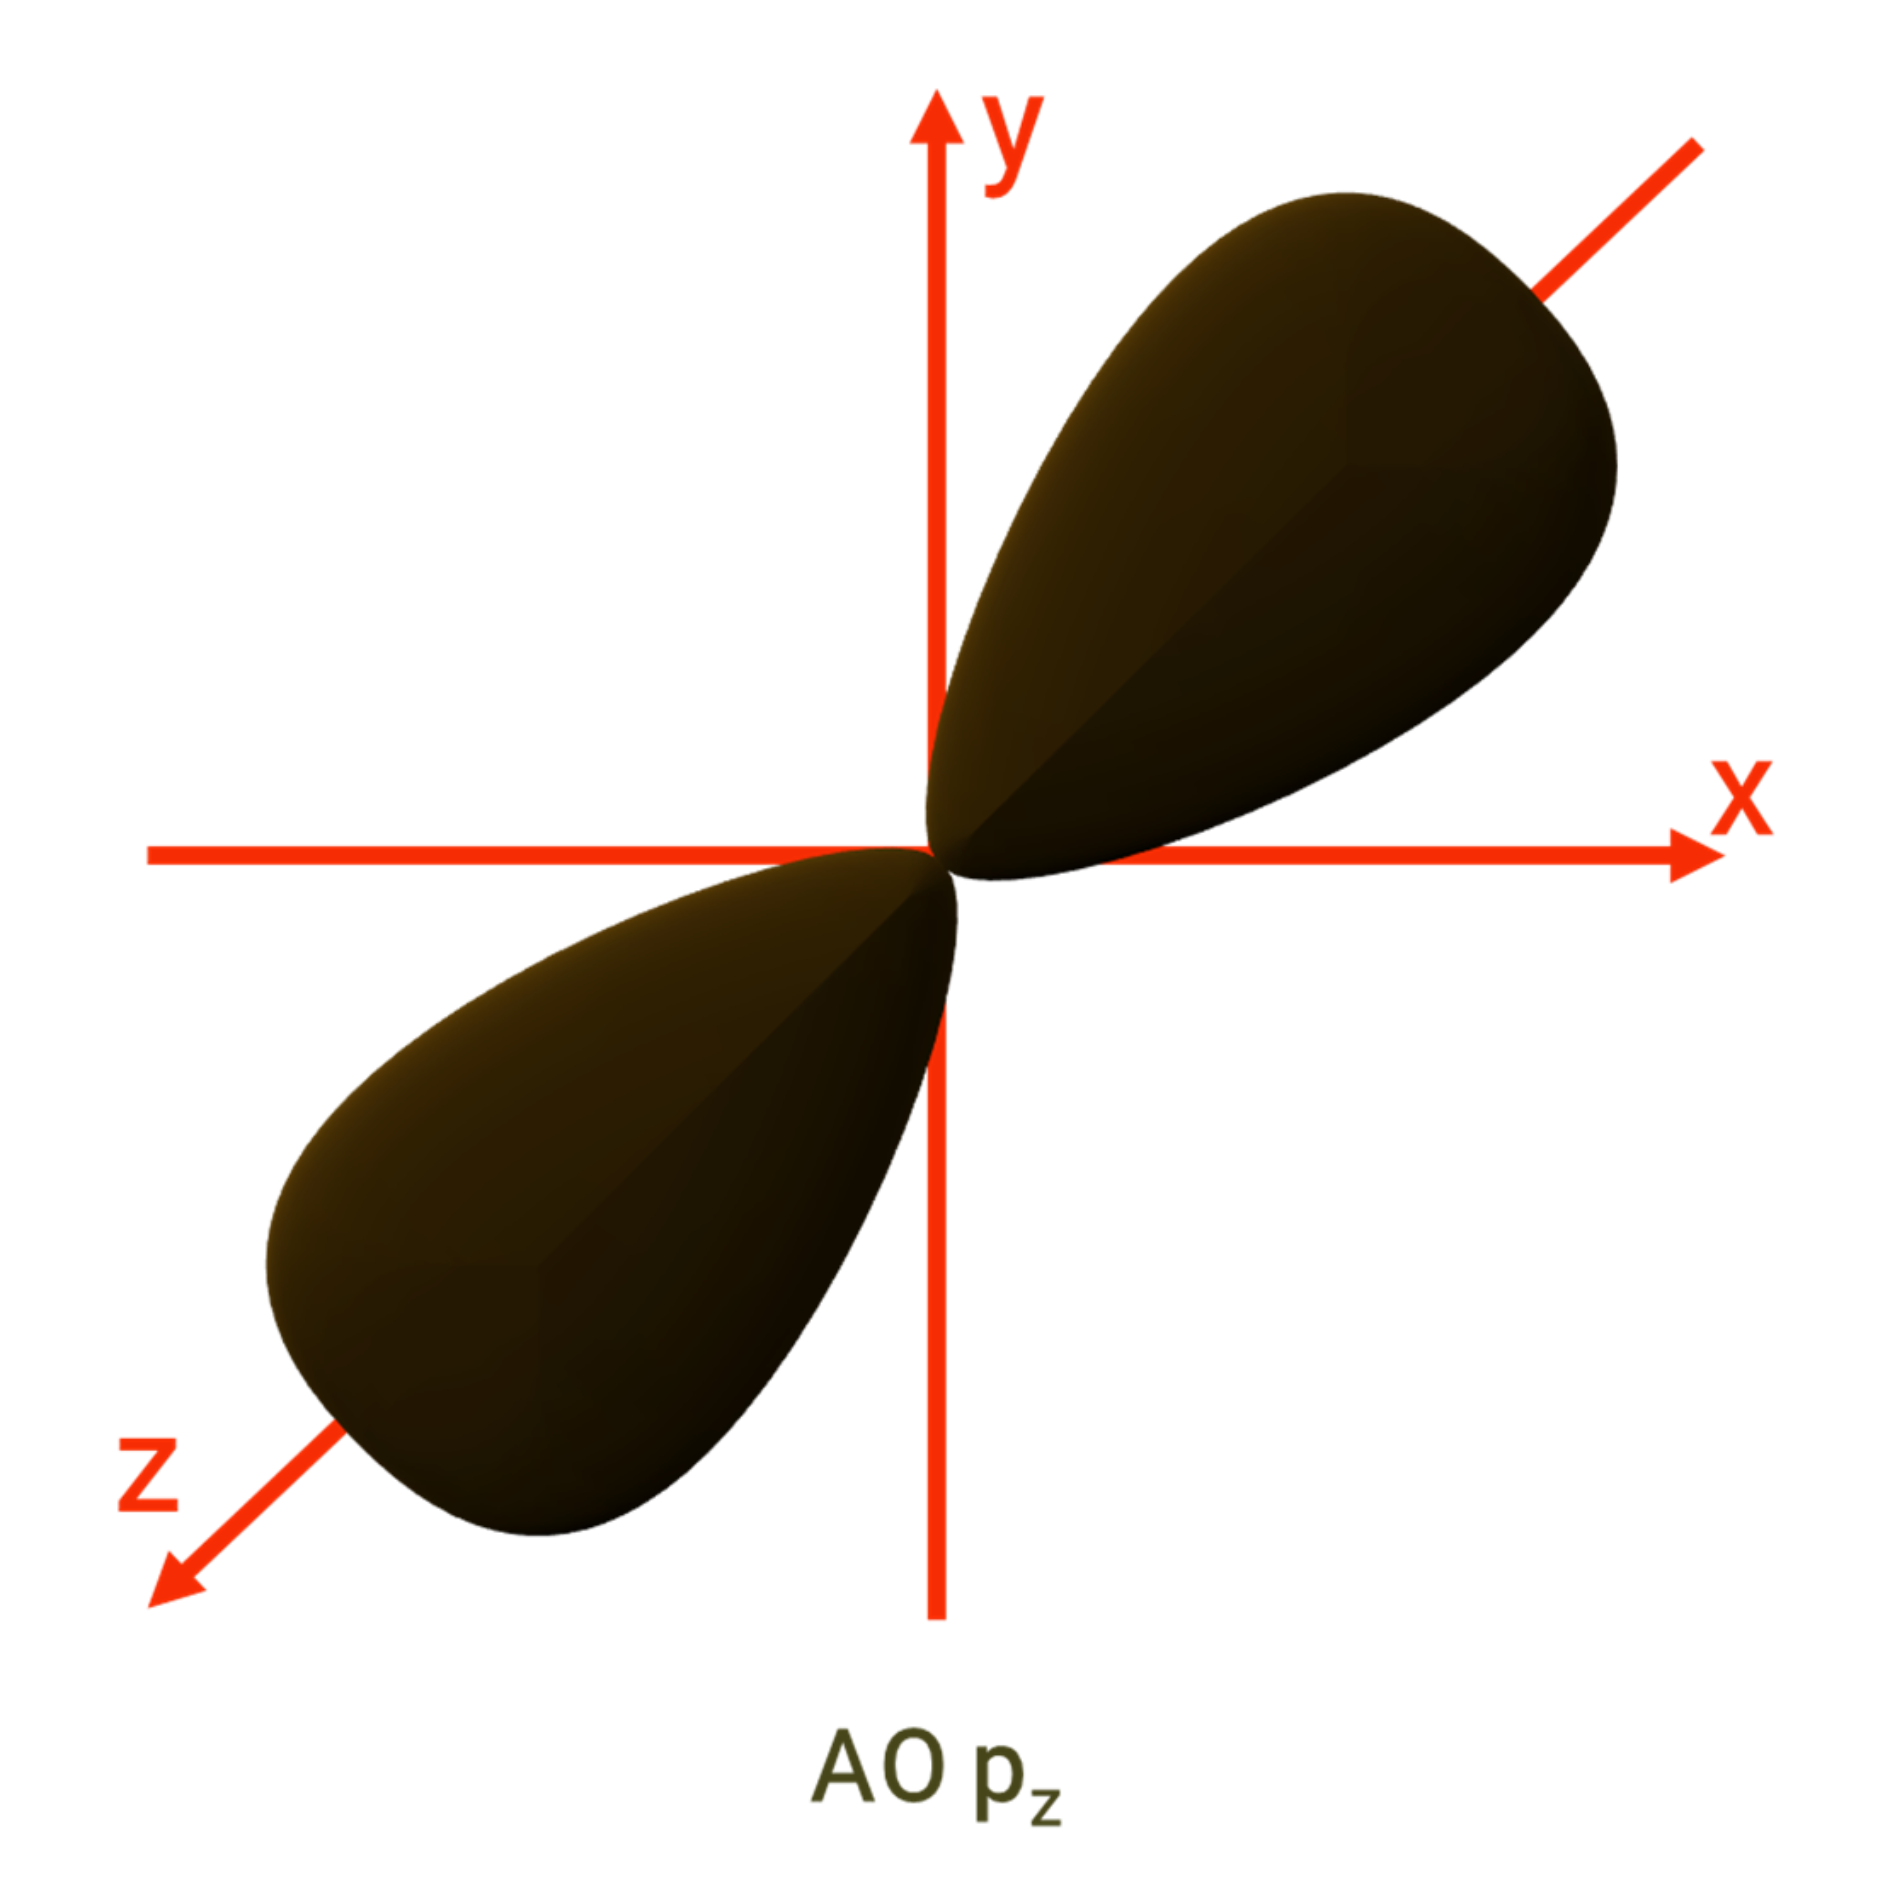
\includegraphics[width=3cm]{Images/anhminhoa/Pz.png}\\ 
	};
\end{tikzpicture}
\captionof{figure}{Hình dạng của các AO-s và AO-d}
\label{fig:hinhdangAO}
\subsection{Lớp và phân lớp electon}
\subsubsection{Lớp electron}

\begin{hoplythuyet}
	\begin{itemize}
	\item Trong nguyên tử, các electron được sắp xếp thành từng lớp ( kí hiệu lần lượt là:K,L,M,N,O,P,Q,...) và phân lớp theo mức năng lượng từ thấp đến cao.
	\item Các electron trên cùng  một lớp có mức năng lượng gần bằng nhau.
	\item Lớp electron gần hạt nhân nhất có năng lượng thấp nhất. càng xa hạt nhân năng lượng càng cao.
\end{itemize}
\end{hoplythuyet}
\begin{center}
	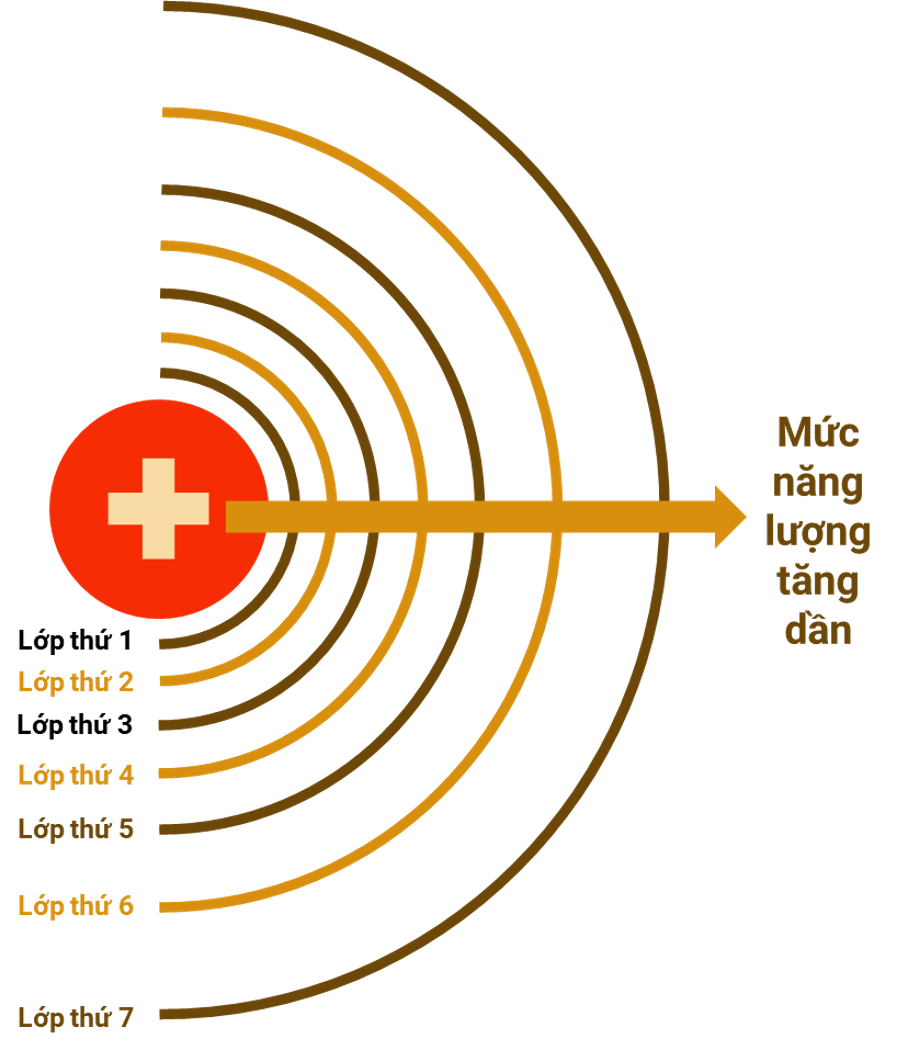
\includegraphics[height=6cm]{Images/anhminhoa/Lopelectron.png}
\end{center}
\subsubsection{Phân lớp electron}
\begin{hoplythuyet}
	\begin{itemize}
		\item Mỗi lớp electron chia thành các phân lớp ( Kí hiệu là: s, p, d, f)
		\item Các electron ở phân lớp s, p, d, f gọi là electron s, p, d, f.
		\item Các electron trên cùng một phân lớp thì có mức năng lượng bằng nhau
		\item Số phân lớp trong mỗi lớp bằng số thứ tự  của lớp đó.
	\end{itemize}
\end{hoplythuyet}

\begin{center}
%%=========Hình 4=========%%
\begin{tikzpicture}[declare function={r=3.0;}]
	\path [fill=cyan](0,0)-- (90:{r+5.6}) arc (90:0:{r+5.6}) -- cycle;
	\path [fill=violet](0,0)-- (90:{r+5.3}) arc (90:0:{r+5.3}) -- cycle;
	\path [fill=\mycolor](0,0)-- (90:{r+5}) arc (90:0:{r+5}) -- cycle;
	\path [fill=\mauphu](0,0) -- (90:{r+4.7}) arc (90:0:{r+4.7}) -- cycle;
	\path [fill=white](0,0)-- (90:{r+4.4}) arc (90:0:{r+4.4}) -- cycle;
	\path [fill=violet](0,0)-- (90:{r+3.6}) arc (90:0:{r+3.6}) -- cycle;
	\path [fill=\mycolor](0,0)-- (90:{r+3.3}) arc (90:0:{r+3.3}) -- cycle;
	\path [fill=\mauphu](0,0) -- (90:{r+3}) arc (90:0:{r+3}) -- cycle;
	\path [fill=white](0,0)-- (90:{r+2.7}) arc (90:0:{r+2.7}) -- cycle;
	\path [fill=\mycolor](0,0)-- (90:{r+2}) arc (90:0:{r+2}) -- cycle;
	\path [fill=\mauphu](0,0)-- (90:{r+1.7}) arc (90:0:{r+1.7}) -- cycle;
	\path [fill=white](0,0) -- (90:{r+1.4}) arc (90:0:{r+1.4}) -- cycle;
	\path [fill=\mauphu](0,0) -- (90:{r+.8}) arc (90:0:{r+.8}) -- cycle;
	\path [fill= white](0,0) -- (90:{r+.5}) arc (90:0:{r+.5}) -- cycle;
	\path [fill=\maunhan](0,0) -- (90:r) arc (90:0:r) -- cycle;
	\path ($(0,0)+(1.5,1.3)$) node[font=\color{white}\bfseries\sffamily,text width =2.5cm] {Hạt nhân nguyên tử};
%	\draw[%
%	decoration={%
%		text along path,
%        text={{\bfseries\sffamily H}{\bfseries\sffamily ử}{\bfseries\sffamily t} {\bfseries\sffamily n}{\bfseries\sffamily h}{\bfseries\sffamily â}{\bfseries\sffamily n} {\bfseries\sffamily n}{\bfseries\sffamily g}{\bfseries\sffamily u}{\bfseries\sffamily y}{\bfseries\sffamily ê}{\bfseries\sffamily n} {\bfseries\sffamily t}{\bfseries\sffamily ử}},
%		text align={center},
%		text color = white
%		},
%		decorate,
%		]
%		(90:{r-.4}) arc(90:0:{r-.4});
	\path 
	(0:{r+0.65}) node[font=\tiny\sffamily,below]{1s}
	(90:{r+0.65}) node[font=\tiny\sffamily,left,anchor=east]{Lớp thứ 1}
	(0:{r+1.55}) node[font=\tiny\sffamily,below]{2s}
	(90:{r+1.7}) node[font=\tiny\sffamily,left,anchor=east]{Lớp thứ 2}
	(0:{r+1.85}) node[font=\tiny\sffamily,below]{2p}
	(0:{r+2.85}) node[font=\tiny\sffamily,below]{3s}
	(0:{r+3.15}) node[font=\tiny\sffamily,below]{3p}
	(90:{r+3.15}) node[font=\tiny\sffamily,left,anchor=east]{Lớp thứ 3}
	(0:{r+3.45}) node[font=\tiny\sffamily,below]{3d}
	(0:{r+3.45}) node[font=\tiny\sffamily,below]{3d}
	(0:{r+4.55}) node[font=\tiny\sffamily,below]{4s}
	(0:{r+4.85}) node[font=\tiny\sffamily,below]{4p}
	(90:{r+5.0}) node[font=\tiny\sffamily,left,anchor=east]{Lớp thứ 4}
	(0:{r+5.15}) node[font=\tiny\sffamily,below]{4d}
	(0:{r+5.45}) node[font=\tiny\sffamily,below]{4f}
	;
\end{tikzpicture}
%%========= Hết hình4=========%
\captionof{figure}{Kí hiệu một số lớp và phân lớp trong nguyên tử}
\end{center}

\begin{center}
\begin{tikzpicture}[font=\normalsize]
	
\tikzset{%
%%Lưu tùy chọn vẽ đường tròn với tên ntdcircle	
ntdcircle/.style={%
	circle,
	fill=\maudam, % Màu và kiểu viền cho hình tròn
	inner sep=0pt,
	minimum size=.3cm % Kích thước hình tròn
},
mycircle/.pic={%
	\node[ntdcircle] at (0,0) {};
},
	%%% Đinh dạng trong 1 ô
	ntdnode/.style={%
		thick,
		anchor=center,
		align=center,
		minimum height = .4cm,
		minimum width = 2cm,
		font=\sffamily,
	},
	%%% Định dạng toàn cục
	ntdmatrix/.style={%
		matrix of nodes,
		inner sep =5pt,
		nodes in empty cells,
		fill =\mycolor!15,
		row sep=-\pgflinewidth,
		column sep=-\pgflinewidth,
		nodes={ntdnode},
		row 1/.style={%
			nodes={%
				fill=\mauphu!40!white,
				text centered,
				font=\bfseries\sffamily,
				draw=white,
%				ultra thick,
				inner sep =12pt
			}
		},
		row 2/.style={%
			nodes={%
				align=center,
				font=\bfseries\sffamily,
				inner sep =5pt,
				fill=\mauphu!20!white
			}
		},
		row 3/.style={%
			nodes={%
				align=center,
				font=\bfseries\sffamily,
				inner sep =5pt,
				fill=\mauphu!20!white
			}
		},
		row 4/.style={%
			nodes={%
				align=center,
				font=\bfseries\sffamily,
				inner sep =5pt,
				fill=\mauphu!40!white
			}
		},
		row 5/.style={%
			nodes={%
				align=center,
				font=\bfseries\sffamily,
				inner sep =5pt,
				fill=\mauphu!40!white
			}
		},
		row 6/.style={%
			nodes={%
				align=center,
				font=\bfseries\sffamily,
				inner sep =5pt,
				fill=\mauphu!20!white
			}
		},
		row 7/.style={%
			nodes={%
				align=center,
				font=\bfseries\sffamily,
				inner sep =5pt,
				fill=\mauphu!20!white
			}
		},
		row 8/.style={%
			nodes={%
				align=center,
				font=\bfseries\sffamily,
				inner sep =5pt,
				fill=\mauphu!40!white
			}
		},
		row 9/.style={%
			nodes={%
				align=center,
				font=\bfseries\sffamily,
				inner sep =5pt,
				fill=\mauphu!40!white
			}
		},
		column 1/.style={%
			nodes={%
				align=center,
				font=\bfseries\sffamily,
				inner sep =5pt
			}
		},
		column 5/.style={%
			nodes={%
				minimum width = 3.5cm,
			}
		},
	}
}

\matrix (ple) [ntdmatrix]{%
	 &  &  &  & \\
	 &  &  &  & \\
	 &  &  &  & \\
	 &  &  &  & \\
	 &  &  &  & \\
	 &  &  &  & \\
	 &  &  &  & \\
	 &  &  &  & \\
	 &  &  &  & \\
};
\fill[%
draw=white,
fill=\mauphu!60!white,
inner sep =5pt
]
(ple-1-1.north west)rectangle (ple-1-1.south east)node[anchor=center,midway,font=\bfseries\sffamily]{Lớp};
\fill[%
draw=white,
fill=\mauphu!60!white,
inner sep =5pt
]
(ple-1-1.north east)rectangle (ple-1-5.south east)node[anchor=center,midway,font=\bfseries\sffamily]{Phân lớp và số Orbital trên phân lớp};

\foreach \j/\n in {3/1s,5/2s,7/3s,9/4s}{%
	\path ([yshift=10pt]ple-\j-2.center) node[font=\sffamily] {\n};
	\foreach \i in {0}{%
		\draw 
		($(ple-\j-2.center)+(\i,0)$) pic{mycircle}
		;
	}

}

\foreach \j/\n in {5/2p,7/3p,9/4p}{%
	\path ([yshift=10pt]ple-\j-3.center) node[font=\sffamily] {\n};
	\foreach \i in {-0.35,0,.35}{%
		\draw 
		($(ple-\j-3.center)+(\i,0)$) pic{mycircle}
		;
	}
	
}

\foreach \j/\n in {7/3d,9/4d}{%
	\path ([yshift=10pt]ple-\j-4.center) node[font=\sffamily] {\n};
	\foreach \i in {-0.7,-0.35,0,.35,0.7}{%
		\draw 
		($(ple-\j-4.center)+(\i,0)$) pic{mycircle}
		;
	}
	
} 

\foreach \j in {9}{%
	\path ([yshift=10pt]ple-\j-5.center) node[font=\sffamily] {4f};
	\foreach \i in {-1.05,-0.7,-0.35,0,.35,0.7,1.05}{%
		\draw 
		($(ple-\j-5.center)+(\i,0)$) pic{mycircle}
		;
	}
} 

\foreach \x/\y/\z/\t in {20/2/3/1,40/4/5/2,20/6/7/3,40/8/9/4}{%
\fill[draw=white,fill=\mauphu!\x!white] (ple-\y-1.north west) rectangle (ple-\z-1.south east) node [anchor=center,midway,font=\bfseries\sffamily]{n=\t};
}

\end{tikzpicture}
\end{center}
\subsubsection{Cấu hình electron}
\paragraph{Nguyên lý vững bền}
\begin{hoplythuyet}
\GSND[\bfseries][\faTrello][\maunhan]{Nguyên lý vững bền}\\
\lq\lq Ở trạng thái cơ bản,các electron trong nguyên tử chiếm lần lượt những Orbital có mức năng lượng từ thấp đến cao.\rq\rq
\end{hoplythuyet}
%%%%%%%%%==============Nguyên lý vững bền==================%%%%%%%%%%
%\begin{center}
%		\begin{tikzpicture}[font=\Large,declare function={d=1.5cm; r={sqrt(2)/8 *d};}]
%			\tikzset{%a
%			ntdnode/.style={%
%				minimum height=0.65cm,
%				align=center,
%				font=\sffamily\bfseries,
%				minimum width =d,
%				minimum height =d,
%%				draw=cyan,
%			},
%			ntdmatrix/.style={%
%				matrix of nodes,
%				inner sep=5pt,
%				nodes in empty cells,
%%				fill=\mycolor!75,
%				row sep=-\pgflinewidth,
%				column sep=-\pgflinewidth,
%				nodes={ntdnode},
%				rounded corners=4pt,
%			},
%			line/.style={%
%			\maunhan!50!red,
%			arrows = {-Stealth},
%			line width=3pt,
%			}
%		}
%
%		\matrix (NLVB) [ntdmatrix] {%
%			 &  &  &  \\
%			 &  &  &  \\
%			 &  &  &  \\
%			 &  &  &  \\
%			 &  &  &  \\
%			 &  &  &  \\
%			 &  &  &  \\
%			 &  &  &  \\
%	};
%	
%	\draw (NLVB-1-1.south west) arc(135:315:r)
%	--(NLVB-1-1.east) arc(135:-45:r)--(NLVB-2-1.north east)
%	--(NLVB-2-1.south west) arc(135:315:r)--(NLVB-1-2.east) arc(135:-45:r)--(NLVB-2-2.north east)
%	--(NLVB-3-1.south west) arc(135:315:r)--(NLVB-2-2.east) arc(135:-45:r)--(NLVB-3-2.north east)
%	--(NLVB-4-1.south west) arc(135:315:r)--(NLVB-2-3.east) arc(135:-45:r)--(NLVB-3-3.north east)
%	--(NLVB-5-1.south west) arc(135:315:r)--(NLVB-3-3.east) arc(135:-45:r)--(NLVB-4-3.north east) 
%	--(NLVB-6-1.south west) arc(135:315:r)--(NLVB-3-4.east) arc(135:-45:r)--(NLVB-4-4.north east)
%	--(NLVB-7-1.south west) arc(135:315:r)--(NLVB-4-4.east) arc(135:-45:r)--(NLVB-5-4.north east)
%	;
%	
%	\foreach \h/\t/\n in {1/1/1,2/1/2,2/2/3,3/2/4,3/3/5,4/3/6,4/4/7,5/4/8}{%
%	\draw[line] (NLVB-\h-\t.north east)--(NLVB-\n-1.south west);	
%	}
%
%	
%	\foreach \i in {1,2,...,8}{%
%		\foreach \j in {1}{%
%			\path(NLVB-\i-\j.center) node[font=\bfseries\Large\sffamily,anchor=center]{\ntdshape{\i \color{\mycolor}{s}}}	;
%		}
%	}
%	\foreach \i in {2,3,...,7}{%
%		\foreach \j in {2}{%
%			\path(NLVB-\i-\j.center) node[font=\bfseries\Large\sffamily,anchor=center]{\ntdshape{\i \color{\maudam}{p}}}	;
%		}
%	}
%	\foreach \i in {3,4,...,6}{%
%		\foreach \j in {3}{%
%			\path(NLVB-\i-\j.center) node[font=\bfseries\Large\sffamily,anchor=center]{\ntdshape{\i \color{\maunhan}{d}}}	;
%		}
%	}
%	\foreach \i in {4,5}{%
%		\foreach \j in {4}{%
%			\path(NLVB-\i-\j.center) node[font=\bfseries\Large\sffamily,anchor=center]{\ntdshape{\i \color{\mauphu}{f}}}	;
%		}
%	}
%		\end{tikzpicture}
%	\captionof{figure}{Quy tắc Klechkowski }
%	\label{fig:Klechkowski}
%\end{center}

\begin{emcobiet}
		Các electron sắp sếp theo thứ tự mức năng lượng từ thấp đến cao được mô phỏng theo \indam{Quy tắc Klechkowski} (Xem hình \ref{fig:Klechkowski})\\
		Theo quy tắc này ta có trật tự mức năng lượng electron như sau:\\
		\begin{center}
		\boxct[\maunhan][3pt][\bfseries\sffamily][arc is angular]{1s,2s,2p,3p,4s,3d,4p,5s,4d,5p,6s,$\ldots$}
		\end{center}
		\begin{center}
			\begin{tikzpicture}[font=\Large,declare function={d=1.5cm; r={sqrt(2)/8 *d};}]
				\tikzset{%a
					ntdnode/.style={%
						minimum height=0.65cm,
						align=center,
						font=\sffamily\bfseries,
						minimum width =d,
						minimum height =d,
						%				draw=cyan,
					},
					ntdmatrix/.style={%
						matrix of nodes,
						inner sep=5pt,
						nodes in empty cells,
%						fill=\mycolor,
						row sep=-\pgflinewidth,
						column sep=-\pgflinewidth,
						nodes={ntdnode},
						rounded corners=4pt,
					},
					line/.style={%
						\maunhan!50!red,
						arrows = {-Stealth},
						line width=3pt,
					}
				}
				
				\matrix (NLVB) [ntdmatrix] {%
					&  &  &  \\
					&  &  &  \\
					&  &  &  \\
					&  &  &  \\
					&  &  &  \\
					&  &  &  \\
					&  &  &  \\
					&  &  &  \\
				};
				
				\draw (NLVB-1-1.south west) arc(135:315:r)
				--(NLVB-1-1.east) arc(135:-45:r)--(NLVB-2-1.north east)
				--(NLVB-2-1.south west) arc(135:315:r)--(NLVB-1-2.east) arc(135:-45:r)--(NLVB-2-2.north east)
				--(NLVB-3-1.south west) arc(135:315:r)--(NLVB-2-2.east) arc(135:-45:r)--(NLVB-3-2.north east)
				--(NLVB-4-1.south west) arc(135:315:r)--(NLVB-2-3.east) arc(135:-45:r)--(NLVB-3-3.north east)
				--(NLVB-5-1.south west) arc(135:315:r)--(NLVB-3-3.east) arc(135:-45:r)--(NLVB-4-3.north east) 
				--(NLVB-6-1.south west) arc(135:315:r)--(NLVB-3-4.east) arc(135:-45:r)--(NLVB-4-4.north east)
				--(NLVB-7-1.south west) arc(135:315:r)--(NLVB-4-4.east) arc(135:-45:r)--(NLVB-5-4.north east)
				;
				
				\foreach \h/\t/\n in {1/1/1,2/1/2,2/2/3,3/2/4,3/3/5,4/3/6,4/4/7,5/4/8}{%
					\draw[line] (NLVB-\h-\t.north east)--(NLVB-\n-1.south west);	
				}
				
				
				\foreach \i in {1,2,...,8}{%
					\foreach \j in {1}{%
						\path(NLVB-\i-\j.center) node[font=\bfseries\Large\sffamily,anchor=center]{\ntdshape{\i \color{\mycolor}{s}}}	;
					}
				}
				\foreach \i in {2,3,...,7}{%
					\foreach \j in {2}{%
						\path(NLVB-\i-\j.center) node[font=\bfseries\Large\sffamily,anchor=center]{\ntdshape{\i \color{\maudam}{p}}}	;
					}
				}
				\foreach \i in {3,4,...,6}{%
					\foreach \j in {3}{%
						\path(NLVB-\i-\j.center) node[font=\bfseries\Large\sffamily,anchor=center]{\ntdshape{\i \color{\maunhan}{d}}}	;
					}
				}
				\foreach \i in {4,5}{%
					\foreach \j in {4}{%
						\path(NLVB-\i-\j.center) node[font=\bfseries\Large\sffamily,anchor=center]{\ntdshape{\i \color{\mauphu}{f}}}	;
					}
				}
			\end{tikzpicture}
			\captionof{figure}{Quy tắc Klechkowski }
			\label{fig:Klechkowski}
		\end{center}
\end{emcobiet}

\paragraph{Nguyên lý pauli}

\begin{hoplythuyet}
	\indam{Nguyên lí Pauli:} Mỗi orbital chỉ chứa tối đa 2 electron và có chiều tự quay ngược nhau.
\end{hoplythuyet}

\begin{tikzpicture}
	\path (0,0) node[anchor=center](eghepdoi) {\Eghepdoi}
	      (eghepdoi.east) node [xshift=-5pt,anchor=west]{:\ \indam{Electron ghép đôi}}
	;
	
	\path (0,-1) node[anchor=center](edocthan) {\Edocthan}
	(edocthan.east) node [xshift=-5pt,anchor=west]{:\ \indam{Electron độc thân}}
	;
\end{tikzpicture}
\paragraph{Xác định số AO và số electron tối đa trong một phân lớp và trong mỗi lớp}

\begin{tikzpicture}[font=\normalsize,declare function={d=2.6cm;r=.9cm;}]
	\tikzset{%a
		ntdnode/.style={%
			align=center,
			font=\sffamily\bfseries,
			minimum width =d,
			minimum height =r,
			draw=white,
			anchor =center,
			fill=\mycolor!75,
		},
		ntdmatrix/.style={%
			matrix of nodes,
			inner sep=5pt,
			nodes in empty cells,
%			fill=\mycolor!15,
			row sep=-\pgflinewidth,
			column sep=-\pgflinewidth,
			nodes={ntdnode},
%			rounded corners=4pt,
		column 1/.style={%
			nodes={%
				align=center,
				font=\bfseries\sffamily,
				inner sep =5pt,
				minimum width =1.2cm
			}
		},
		row 1/.style={%
			nodes={%
				align=center,
				font=\color{white}\bfseries\sffamily,
				inner sep =5pt,
				minimum height =2cm,
				fill=\maudam!85
			}
		},		
		column 4/.style={%
			nodes={%
				minimum width =3.4cm
			}
		},
		column 5/.style={%
			nodes={%
				minimum width =3.8cm
			}
		},
		column 6/.style={%
			nodes={%
				minimum width =3.6cm
			}
		},	
	},
		line/.style={%
			\maunhan!50!red,
			arrows = {-Stealth},
			line width=3pt,
		}
	}
	\matrix (soelectron) [ntdmatrix] {%
	n	& Tên lớp & \makecell{Tên \\phân lớp} & \makecell{Số AO\\ trong mỗi\\ phân lớp} & \makecell{Số e \\tối đa trong\\ mỗi phân lớp} & \makecell[c]{Số e \\tối đa trong\\ một lớp} \\
		&  & s & 1 & 2 &  \\
		&  & s & 1 & 2 &  \\
		&  & p & 3 & 6 &  \\
		&  & s & 1 & 2 &  \\
		&  & p & 3 & 6 &  \\
		&  & d &  5& 10& \\
		&  & s & 1 & 2 &  \\
		&  & p & 3 & 6 &  \\
		&  & d & 5 & 10&  \\
		&  & f & 7 & 14&  \\
	n	&  & $n^2$ &   & &  \\
	};
\foreach \i/\j/\k in {2/2/1,3/4/2,5/7/3,8/11/4,12/12/n}{%
\path[draw=white,fill=\mycolor!75](soelectron-\i-1.north west) rectangle (soelectron-\j-1.south east)node[midway,anchor=center]{\indam{\k}};
}	

\foreach \i/\j/\k in {2/2/K,3/4/L,5/7/M,8/11/N}{%
	\path[draw=white,fill=\mycolor!75](soelectron-\i-2.north west) rectangle (soelectron-\j-2.south east)node[midway,anchor=center]{\indam[black]{\k}};
}

\foreach \i/\j/\k in {2/2/$2=2\cdot1^2$,3/4/$8=2\cdot2^2$,5/7/$18=2\cdot3^2$,8/11/$32=2\cdot4^2$,12/12/$2n^2$}{%
	\path[draw=white,fill=\mycolor!75](soelectron-\i-6.north west) rectangle (soelectron-\j-6.south east)node[midway,anchor=center]{\indam[black]{\k}};
}
\path[draw=white,fill=\mycolor!75](soelectron-12-2.north west) rectangle (soelectron-12-5.south east)node[midway,anchor=center]{\indam[black]{$n^2$}};	
\end{tikzpicture}
\paragraph{Quy tắc hund}
\begin{hoplythuyet}
	\lq \lq Trong cùng một phân lớp chưa bão hòa, các electron sẽ phân bố vào các AO sao cho số e độc thân là tối đa\rq \rq
\end{hoplythuyet}


\begin{hoivadap}
	Trong các trường hợp dưới đây trường hợp nào các electron điền e vào các orbital theo các nguyên lý và quy tắc đã học
\begin{myenum}
	\item
	\begin{adjustbox}{valign=m}
		\begin{tikzpicture}[declare function={x=.896cm;l=1.2;}]   
			\path(0:{0*x}) node [anchor=center](dxy) {\Eghepdoi}
			(0:{1*x}) node [anchor=center](dyz) {\Eghepdoi}
			(0:{2*x}) node [anchor=center](dzz) {\Eghepdoi}
			(0:{3*x}) node [anchor=center](pxxyy) {\Eghepdoi}
			(0:{4*x}) node [anchor=center](pxz) {\Edocthan};
			\path (0:{5*x}) node [anchor=center,transform canvas={shift={(10pt,-3pt)}}](ssss) {\Edocthan[\maunhan]};
			\path([xshift=15pt]ssss.south)node[anchor=north]{$4s^1$};
			\path([xshift=3.2pt]dzz.south)node[anchor=north]{$3d^{9}$};
		\end{tikzpicture}
	\end{adjustbox}
	\item
	\begin{adjustbox}{valign=m}
		\begin{tikzpicture}[declare function={x=.896cm;l=1.2;}]  
			\path(0:{0*x}) node [anchor=center](dxy) {\Eghepdoi}
			(0:{1*x}) node [anchor=center](dyz) {\Eghepdoi}
			(0:{2*x}) node [anchor=center](dzz) {\Edocthan}
			(0:{3*x}) node [anchor=center](pxxyy) {\Edocthan}
			(0:{4*x}) node [anchor=center](pxz) {\Edocthan};
			\path (0:{5*x}) node [anchor=center,transform canvas={shift={(10pt,-3pt)}}](ssss) {\Eghepdoi[\maunhan]};
			\path([xshift=15pt]ssss.south)node[anchor=north]{$4s^2$};
			\path([xshift=3.2pt]dzz.south)node[anchor=north]{$3d^{9}$};
		\end{tikzpicture}
	\end{adjustbox}
	\item
	\begin{adjustbox}{valign=m}
		\begin{tikzpicture}[declare function={x=.896cm;l=1.2;}]  
			\path(0:{0*x}) node [anchor=center](SSS) {\Eghepdoi}
			(0:{1*x}) node [anchor=center,transform canvas={shift={(10pt,3pt)}}](p) {\Eghepdoi}
			(0:{2*x}) node [anchor=center,transform canvas={shift={(10pt,3pt)}}](pp) {\Eghepdoi}
			(0:{3*x}) node [anchor=center,transform canvas={shift={(10pt,3pt)}}](ppp) {\AOtrong};
			\path([xshift=5pt]SSS.south)node[anchor=north]{$3s^2$};
			\path([xshift=14pt]pp.south)node[anchor=north]{$3p^{4}$};
		\end{tikzpicture}
	\end{adjustbox}
\end{myenum}
\end{hoivadap}

\begin{notegsnd}
%%%%=================== Phan lop d========================%%%%%%%%%%%%%
\begin{tikzpicture}[declare function={d=.6cm;r={d/2.4};}]
		\tikzset{
			eghepdoi/.pic={
				\draw[arrows={-Stealth}, line width=1pt, \maudam]
				(0,0)--(0,d);
				\draw[arrows={-Stealth}, line width=1pt, \maudam]
				(r,d)--(r,0);
			},
			edocthan/.pic={
				\draw[arrows={-Stealth}, line width=1pt, \maudam]
				(0,0)--(0,d);
			},
			echuaghepdoi/.pic={
				\draw[arrows={-Stealth}, line width=1pt, \maudam]
				(0,0)--(0,d);
				\path[arrows={-Stealth}, line width=1pt, \maudam]
				(r,d)--(r,0);
			}
		}
%%%%%%%%%%%%%%%%%%%%%%%Cấu hình 3d bão hòa%%%%%%%%%%%%%%%%%%%%%%%%%%%%%%
	\matrix (pld)[%
	matrix of nodes,
	nodes={%
		draw= \maudam,
		thick,
		minimum height =.8cm,
		minimum width = .8cm,
		anchor = center,
		align =center,
		inner sep =3pt,
	},
	nodes in empty cells,
	row sep=-\pgflinewidth,
	column sep=-\pgflinewidth,
	]{%
		& & & &\\
	};
%%%%%%%%%%%%%%%%%%%%%%%%%%%%%%%%%%%%%%%%%%%%%%%%%%%%%%%%%%%%%%%%%%%%%%%%%%%%%%%%	
	\begin{scope}[transform canvas={xshift=-3.7pt,yshift=-8.7pt}]
	\foreach \x in {1,2,3,4,5}{
		\draw(pld-1-\x.center) pic {eghepdoi};
	}
\end{scope}	

\path (pld.south) node[anchor=north,font=\small] {Cấu hình bão hòa (bền)};
	\end{tikzpicture}
%%%%%%%%%%%%%%%%%%%%%%%%Cấu hình 3d Bán bão hòa=======================%%%%%%%%%%%%%%%%%%%%%%%%	
	\begin{tikzpicture}[declare function={d=.60cm;r={d/2.4};}]
	\tikzset{
		eghepdoi/.pic={
			\draw[arrows={-Stealth}, line width=1pt, \maudam]
			(0,0)--(0,d);
			\draw[arrows={-Stealth}, line width=1pt, \maudam]
			(r,d)--(r,0);
		},
		edocthan/.pic={
			\draw[arrows={-Stealth}, line width=1pt, \maudam]
			(0,0)--(0,d);
		},
		echuaghepdoi/.pic={
			\draw[arrows={-Stealth}, line width=1pt, \maudam]
			(0,0)--(0,d);
			\path[arrows={-Stealth}, line width=1pt, \maudam]
			(r,d)--(r,0);
		}
	}
	%%%%%%%%%%%%%%%%%%%%%%%%%%%%%%%%%%%%%%%%%%%%%%%%%%%%%%%%%%%%%%%%%%%%%%%%%%%%%%%%
	\matrix (pld)[%
	matrix of nodes,
	nodes={%
		draw= \maudam,
		thick,
		minimum height =.8cm,
		minimum width = .8cm,
		anchor = center,
		align =center,
		inner sep =3pt,
	},
	nodes in empty cells,
	row sep=-\pgflinewidth,
	column sep=-\pgflinewidth,
	]{%
		& & & &\\
	};
	%%%%%%%%%%%%%%%%%%%%%%%%%%%%%%%%%%%%%%%%%%%%%%%%%%%%%%%%%%%%%%%%%%%%%%%%%%%%%%%%	
	\begin{scope}[transform canvas={xshift=-0.5pt,yshift=-8.7pt}]
		\foreach \x in {1,2,3,4,5}{
			\draw(pld-1-\x.center) pic {edocthan};
		}
	\end{scope}	
\path (pld.south) node[anchor=north,font=\small] {Cấu hình bán bão hòa (bền)};	
\end{tikzpicture}	
%%%%%%%%%%%%%%%%%%%%%%%%Cấu hình 3d chưa bão hòa=======================%%%%%%%%%%%%%%%%%%%%%%%%	
\begin{tikzpicture}[declare function={d=.60cm;r={d/2.4};}]
	\tikzset{
		eghepdoi/.pic={
			\draw[arrows={-Stealth}, line width=1pt, \maudam]
			(0,0)--(0,d);
			\draw[arrows={-Stealth}, line width=1pt, \maudam]
			(r,d)--(r,0);
		},
		edocthan/.pic={
			\draw[arrows={-Stealth}, line width=1pt, \maudam]
			(0,0)--(0,d);
		},
		echuaghepdoi/.pic={
			\draw[arrows={-Stealth}, line width=1pt, \maudam]
			(0,0)--(0,d);
			\path[arrows={-Stealth}, line width=1pt, \maudam]
			(r,d)--(r,0);
		}
	}
	%%%%%%%%%%%%%%%%%%%%%%%%%%%%%%%%%%%%%%%%%%%%%%%%%%%%%%%%%%%%%%%%%%%%%%%%%%%%%%%%
	\matrix (pld)[%
	matrix of nodes,
	nodes={%
		draw= \maudam,
		thick,
		minimum height =.8cm,
		minimum width = .8cm,
		anchor = center,
		align =center,
		inner sep =3pt,
	},
	nodes in empty cells,
	row sep=-\pgflinewidth,
	column sep=-\pgflinewidth,
	]{%
		& & & &\\
	};
	%%%%%%%%%%%%%%%%%%%%%%%%%%%%%%%%%%%%%%%%%%%%%%%%%%%%%%%%%%%%%%%%%%%%%%%%%%%%%%%%	
	\begin{scope}[transform canvas={xshift=-3pt,yshift=-8.7pt}]
		\foreach \x in {1,2,3}{
			\draw(pld-1-\x.center) pic {eghepdoi};
		}
	\end{scope}	
	\begin{scope}[transform canvas={xshift=-0.5pt,yshift=-8.7pt}]
			\foreach \x in {4,5}{
			\draw(pld-1-\x.center) pic {edocthan};
		}
	\end{scope}
	\path (pld.south) node[anchor=north,font=\small] {Cấu hình chưa bão hòa (kém bền)};	
\end{tikzpicture}
\GSND[][\faBell][\maunhan]{Một số cấu hình đặc biệt: ${}_{29}Cu$	và ${}_{24}Cr$}
\begin{itemize}
\item Cấu hình của ${}_{29}Cu$ theo quy luật sẽ là $[Ar]3d^94s^2$ [\footnote{Cách viết cấu hình thu gọn}].Tuy nhiên một electron từ phân lớp 4s tham gia ghép đôi với 1 e độc thân ở 3d để đạt trạng thái bão hào ở phân lớp 3d $[Ar]3d^{10}4s^1$ bền vững hơn.\\
\begin{tikzpicture}	[declare function={x=.896cm;l=1.2;}]	
	\path(0:{0*x}) node [anchor=center](dxy) {\Eghepdoi}
	(0:{1*x}) node [anchor=center](dyz) {\Eghepdoi}
	(0:{2*x}) node [anchor=center](dzz) {\Eghepdoi}
	(0:{3*x}) node [anchor=center](pxxyy) {\Eghepdoi}
	(0:{4*x}) node [anchor=center](pxz) {\Ecbghepdoi[\maunhan]}
	;
	\path([xshift=3.2pt]dzz.south)node[anchor=north]{$3d^9$};
	\begin{scope}[transform canvas={shift={(10pt,-3pt)}}]
		\path (0:{5*x}) node [anchor=center](ssss) {\Eghepdoi[\maunhan]};
		\path([xshift=3.2pt]ssss.south)node[anchor=north]{$4s^2$};
	\end{scope}
	\path(0:{9*x}) node [anchor=center](dxy1) {\Eghepdoi}
	(0:{10*x}) node [anchor=center](dyz1) {\Eghepdoi}
	(0:{11*x}) node [anchor=center](dzz1) {\Eghepdoi}
	(0:{12*x}) node [anchor=center](pxxyy1) {\Eghepdoi}
	(0:{13*x}) node [anchor=center](pxz1) {\Eghepdoi[\maunhan]}
	;
	\path([xshift=3.2pt]dzz1.south)node[anchor=north]{$3d^{10}$};
	\begin{scope}[transform canvas={shift={(10pt,-3pt)}}]
		\path (0:{14*x}) node [anchor=center](ssss1) {\Ecbghepdoi[\maunhan]};
		\path([xshift=3.2pt]ssss1.south)node[anchor=north]{$4s^1$};
	\end{scope}
%	\draw[->,arrows={-Stealth}, line width=1pt]([xshift=16pt]ssss.east)--(dxy1.west);
	\draw[->,arrows={-Stealth}, line width=1pt]([xshift=16pt]ssss.east)--(dxy1.west);
	\draw[\maunhan,->,arrows={-Stealth}, line width=1pt]([xshift=.6cm,yshift=-2pt]ssss.north) .. controls+(90:l) and +(90:l) .. ([xshift=10pt]pxz.north);
\end{tikzpicture}\\
\item Cấu hình của ${}_{24}Cr$:Tương tự như vậy cấu hình đúng của Cr là $[Ar]3d^{5}4s^{1}$ (cấu hình bán bão hòa) thay vì $ [Ar]3d^{4}4s^{2}$\\
\begin{tikzpicture}	[declare function={x=.896cm;l=1.2;}]	
	\path(0:{0*x}) node [anchor=center](dxy) {\Edocthan}
	(0:{1*x}) node [anchor=center](dyz) {\Edocthan}
	(0:{2*x}) node [anchor=center](dzz) {\Edocthan}
	(0:{3*x}) node [anchor=center](pxxyy) {\Edocthan}
	(0:{4*x}) node [anchor=center](pxz) {\AOtrong[\maunhan][.633cm]}
	;
	\path([xshift=3.2pt]dzz.south)node[anchor=north]{$3d^4$};
	\begin{scope}[transform canvas={shift={(10pt,-3pt)}}]
		\path (0:{5*x}) node [anchor=center](ssss) {\Eghepdoi[\maunhan]};
		\path([xshift=3.2pt]ssss.south)node[anchor=north]{$4s^2$};
	\end{scope}
	\path(0:{9*x}) node [anchor=center](dxy1) {\Edocthan}
	(0:{10*x}) node [anchor=center](dyz1) {\Edocthan}
	(0:{11*x}) node [anchor=center](dzz1) {\Edocthan}
	(0:{12*x}) node [anchor=center](pxxyy1) {\Edocthan}
	(0:{13*x}) node [anchor=center](pxz1) {\Edocthan[\maunhan]}
	;
	\path([xshift=3.2pt]dzz1.south)node[anchor=north]{$3d^{5}$};
	\begin{scope}[transform canvas={shift={(10pt,-3pt)}}]
		\path (0:{14*x}) node [anchor=center](ssss1) {\Ecbghepdoi[\maunhan]};
		\path([xshift=3.2pt]ssss1.south)node[anchor=north]{$4s^1$};
	\end{scope}
	%	\draw[->,arrows={-Stealth}, line width=1pt]([xshift=16pt]ssss.east)--(dxy1.west);
	\draw[->,arrows={-Stealth}, line width=1pt]([xshift=16pt]ssss.east)--(dxy1.west);
	\draw[\maunhan,->,arrows={-Stealth}, line width=1pt]([xshift=.6cm,yshift=-2pt]ssss.north) .. controls+(90:l) and +(90:l) .. ([xshift=5pt]pxz.north);
\end{tikzpicture}
\end{itemize}
\end{notegsnd}
\paragraph{Cách viết cấu hình electron nguyên tử}
\begin{dngsnd}
	Cấu hình electron nguyên tử biểu diễn sự phân bố electron trong vỏ nguyên tử trên các phân lớp thuộc các lớp khác nhau.
	
	%%=========Hình 1=========%%
	\begin{center}
		\begin{tikzpicture}[declare function={b=4cm;r=5cm;l=5cm;}]
			\tikzstyle{mynote} = [%
			anchor=center,
			rectangle,
			inner sep =3pt,
			draw =\mycolor, 
			ultra thick,
			rounded corners =4pt,
			text width =3cm,
			align=center,
			font=\large\color{\mycolor!50!black}\bfseries\sffamily
			]
			\tikzstyle{line} = [%
			->,
			arrows={-Stealth},
			line width = 3pt,
			\maudam
			]
			%%%%%%%%%%%%%%%%%%%%%%%%%%%%%%%%%%%%%%%%%%%%%%%%%%%%%%%%%%%%%%%%%
			\path (0,0) coordinate (A) 			node[anchor=center,font=\fontsize{45pt}{6pt}\fontfamily{qag}\selectfont](cauhinh){\indam{1s$^{2}$}}
			  (cauhinh)--++(0:r) coordinate (B)
			  ([yshift=-3pt]cauhinh)--++(180:l) coordinate (C)
			  ([xshift=3pt]cauhinh)--++(-90:b) coordinate (D);
				\path (B) node [mynote,text width =3cm](soe) {Số e trên phân lớp};
				\draw[line] (soe) -- (cauhinh);
			\path (C) node [mynote,text width =2.5cm](Stt) {Số thứ tự lớp};
			\draw[line](Stt)--([yshift=-8pt]cauhinh) ;
				\path (D) node [mynote,text width =2.5cm](KH) {Kí hiệu phân lớp};			
			\draw[line](KH.north)--([xshift=3pt]cauhinh.south);
		\end{tikzpicture}
	\end{center}
	%%========= Hết hình1=========%
\end{dngsnd}
	
\GSND[\bfseries\sffamily][\faArchive][\maunhan]{Quy ước:}
\begin{itemize}
	\item Số thứ tự electron dduocj ghi bằng chữ số (1,2,3,\ldots)
	\item Phân lớp được ghi  bằng các chữ cái thường (s, p, d, f)
	\item Số electron trong một phân lớp được ghi bằng số ở phía trên bên phải của phân lớp ($s^2$,$p^6$,\ldots)
\end{itemize}

\begin{hoplythuyet}
\GSND[\bfseries\sffamily][\faBook][\maunhan]{Cách viết cấu hình electron}	
	\begin{enumerate}[label=\protect{\bfseries\sffamily Bước \arabic*:},wide=0.65cm,leftmargin=0.65cm]
		\item Xác định số electron của nguyên tử
		\item Các electron được phân bố theo thứ tự các AO có mức năng lượng tăng dần, theo các nguyên lý và quy tắc phân bố electron trong nguyên tử
		\item Viết cấu hình electron theo thứ tự các phân lớp trong một lớp và theo thứ tự của các lớp electron.
	\end{enumerate}
\end{hoplythuyet}

\paragraph{Đặc điểm cấu hình electron lớp ngoài cùng của các nguyên tố nhóm A}

\begin{hoplythuyet}
	\begin{itemize}
		\item Các nguyên tử có \indam{1,2,3 electron} ở lớp ngoài cùng thường là các \indam{kim loại} có khuynh hướng nhường đi 1,2,3 electron đó.
		\item Các nguyên tử có \indam{5,6,7 electron} ở lớp ngoài cùng thường là các \indam{phi kim}, có khuynh hướng nhận thêm 3,2,1 electron đó.
		\item Các nguyên tử có \indam{4 electron}  ở lớp ngoài cùng thường là các kim, loạicó thể là \indam{kim loại hoặc phi kim}.
		\item các nguyên tử có \indam{8 electron} ở lớp ngoài cùng là nguyên tử của nguyên tố \indam{khí hiếm} (trừ He có 2 electron ở lớp ngoài cùng) 
	\end{itemize}
\end{hoplythuyet}

